\section{Architecture}
\label{sec:rvos_architecture}

\subsection{Feature Extraction}
As illustrated in Figure \ref{fig:VLFormer}, the input of our framework consists of a image $I$ and a referring expression with $L$ words. 

\textbf{Visual Encoder.}
    For an image, $I \in \mathbb{R}^{H \times W \times 3}$, we extract the multi-scale feature maps by a visual encoder. The visual encoder, e.g., ResNet, usually processes an image with five different stages that correspond to different scales: $1/2$, $1/4$, $1/8$, $1/16$, and $1/32$. 

In our model, we utilize the four last stages and transform their feature dimension into a common dimension $C$ by a Multilayer Perceptron (MLP) module for convenience. We obtain the multi-scale feature maps $\{F_v^j\} \in \mathbb{R}^{\frac{H}{2^j} \times \frac{W}{2^j} \times C}$ for each stage $j \in (2, 3, 4, 5)$, respectively.    
Note that the $H$ and $W$ are the height and width of the original image.

\textbf{Text Encoder.} 
On such referring segmentation problems, the text query usually contains the information about the category, position on the image and appearance of the object. In some cases, the related position between the referred object and others is mentioned. 

CLIP models are learned from a wide range of visual concepts followed by the natural language. Hence, these models are able to capture the information related to the visual concepts better. 

We adopt the text encoder of the CLIP ~\cite{radford_learning_2021} model to extract the linguistic features $F_t \in \mathbb{R}^{L \times C'}$ from the $L$-word expression. 
The text encoder of the CLIP model is a modified Transformer module. 
% Each word of the expression is converted into a token in a 49,252-vocab dictionary.   
For convenience in later stages (e.g., Transformer decoder), we compress the dimension $C'$ to $C$ by a MLP module so that the dimension of linguistic features is now the same as the visual features.
We also add a sinusoidal 1D positional encoding $e_{pos} \in \mathbb{R}^{L \times C} $ to the linguistic features to store the positional information in these features.

% As illustrated in Figure \ref{fig:VLFormer}, the input of our framework consists of a video $V$ and a referring expression with $L$ words. 

% \subsubsection{Visual Encoder}
% For a video with $T$ frames, $V \in \mathbb{R}^{T \times H \times W \times 3}$, we extract the multi-scale feature maps for each frame in the video independently by a visual encoder. The visual encoder (such as ResNet, SwinTransformer,...) usually extracts an image with five different stages that correspond to different scales: $1/2$, $1/4$, $1/8$, $1/16$ and $1/32$. 

% In our model, we utilize the three last stages and transform their feature dimension into a common dimension $C$ for convenience. We obtain the multi-scale feature maps $\{F^i_j\}^T_{i = 1} \in \mathbb{R}^{\frac{H}{2^j} \times \frac{W}{2^j} \times C}$ for each frame $i$ and stage $j \in (3, 4, 5)$.    
% Note that the $H$ and $W$ are the height and width of the original frame.

% \subsubsection{Text Encoder}

% On such referring segmentation problems, the text query usually contains the information about the category, position on the image and appearance of the object. In some cases, the related position between the referred object and others is mentioned. 

% CLIP models are learned from a wide range of visual concepts followed by the natural language. Hence, these models are able to capture the information related to the visual concepts better. 

% We adopt the textual encoder of the CLIP model to extract the linguistic features $F_t \in \mathbb{R}^{L \times C'}$ from the $L$-word expression. 
% The textual encoder of CLIP model is a modified Transformer module. 
% % Each word of the expression is converted into a token in a 49,252-vocab dictionary.   
% For convenience in later stages (Transformer decoder), we compress the dimension $C'$ to $C$ by a MLP module, so that the dimension of linguistic features is now the same as the visual features.


\subsection{Cross-modal Pixel Decoder}
% The multi-scale visual features that are extracted by the backbone will incorporate with the linguistics features, aiming to enrich the information related to the referred object in each frame of the video. Then will be decoded again into the fine-grained features.

% Firstly, the visual features are fused with the linguistic features ${F_t}$, extracted by the text encoder to perform an early interaction between visual and linguistic features by a Visual-Linguistic Early Fusion block (VLEF) for highlighting regions that are matched with the referring expressions. 
% \begin{equation}
%     \hat{F}_v^i = F_v^i \odot MSA(F_v^iW^Q, F_tW^K, F_tW^V)
% \end{equation}
% where MSA(q, k, v) is the multi-head attention layer and $W^Q$, $W^K$, $W_V$ $\in \mathbb{R}^{C \times d_{head}}$ are learnable parameters. This multi-head attention layer is used as a compatibility weight between the visual features and linguistic features. And then, we multiply this weight with the visual feature to focus on region high related to referring expressions. 

% The rest of Pixel Decoder is adopted from Mask2Former\cite{cheng_masked-attention_2022} with a multi-scale deformable attention module to produce a multi-scale features map  for video frames. 

The multi-scale visual features that are extracted by the visual encoder then are incorporated with the linguistics features, aiming to enrich the information related to the referred object in each frame of a video. Then will be gradually decoded again into the fine-grained features.


\begin{figure}[t]
    \centering
    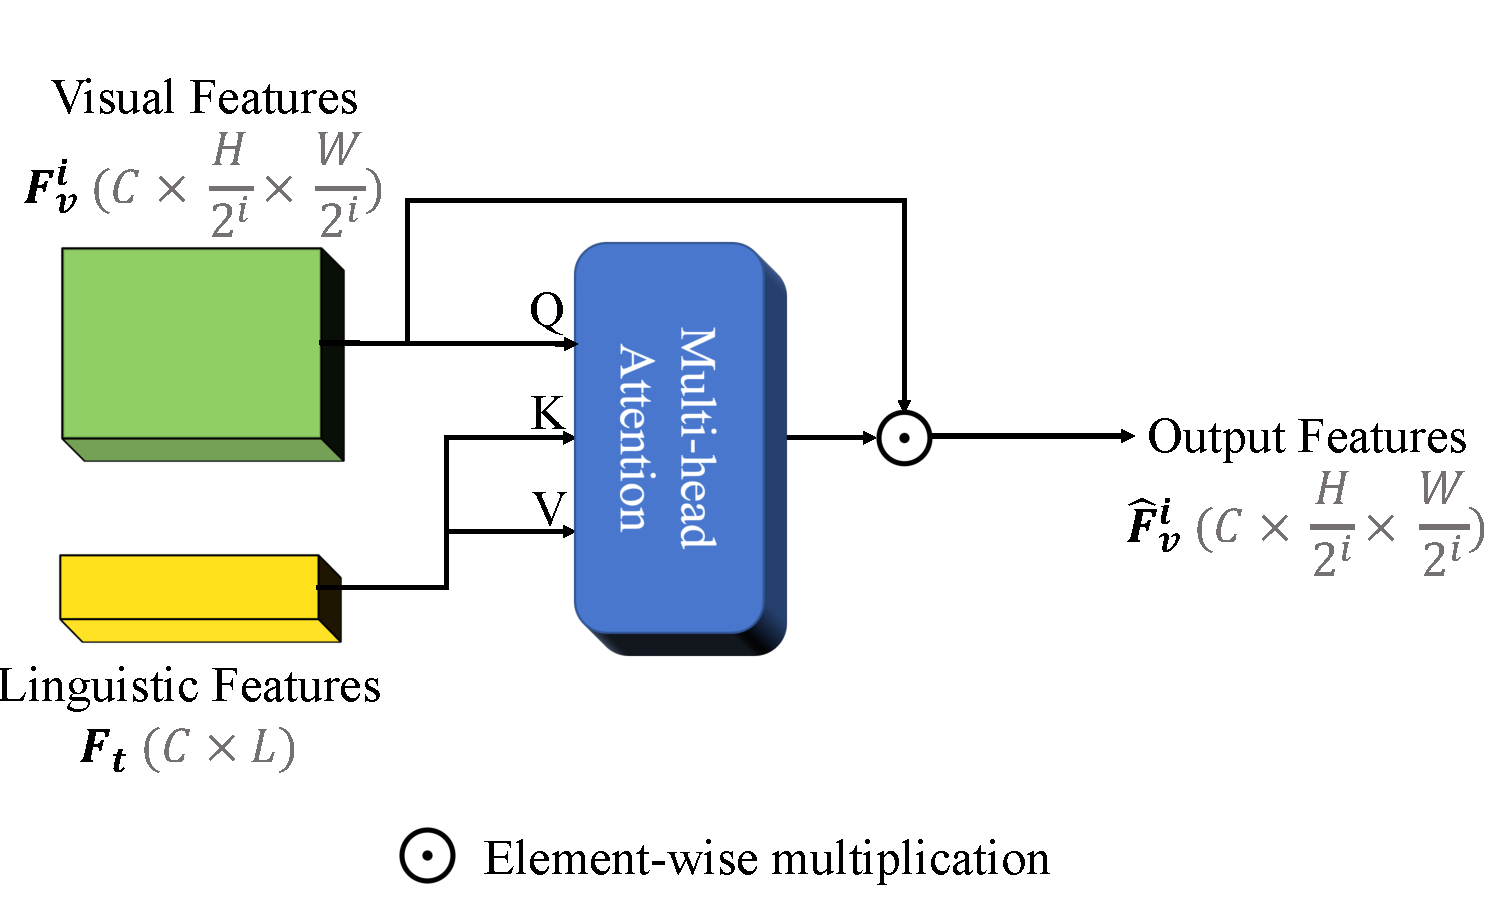
\includegraphics[width=\textwidth]{content/resources/images/referring_segmentation/Language Guidance Module.pdf}
    \caption{The implementation of Language Guidance Module. Visual features $F_v^i$ and linguistic features $F_t$ is used as input to output the language-guided visual features $\hat{F}_v^i$.}
    \label{fig:lgm}
\end{figure} 

\textbf{Language Guidance Module.} 
Firstly, the visual features are fused with the linguistic features ${F_t}$, extracted by the text encoder to perform an early interaction between visual and linguistic features by a Language Guidance Module (LGM) for highlighting regions that are matched with the referring expressions. 
\begin{equation}
    \hat{F}_v^i = F_v^i \odot MSA(F_v^iW^Q, F_tW^K, F_tW^V),
\end{equation}
where MSA(q, k, v) is the multi-head attention layer and $W^Q$, $W^K$, $W_V$ $\in \mathbb{R}^{C \times d_{head}}$ are learnable parameters. This multi-head attention layer is used as a compatibility weight between the visual features and linguistic features. Then, this weight is multiplied with the visual feature to focus on region highly related to referring expressions. Figure \ref{fig:lgm} shows the LGM implementation.


\begin{figure}[t]
    \centering
    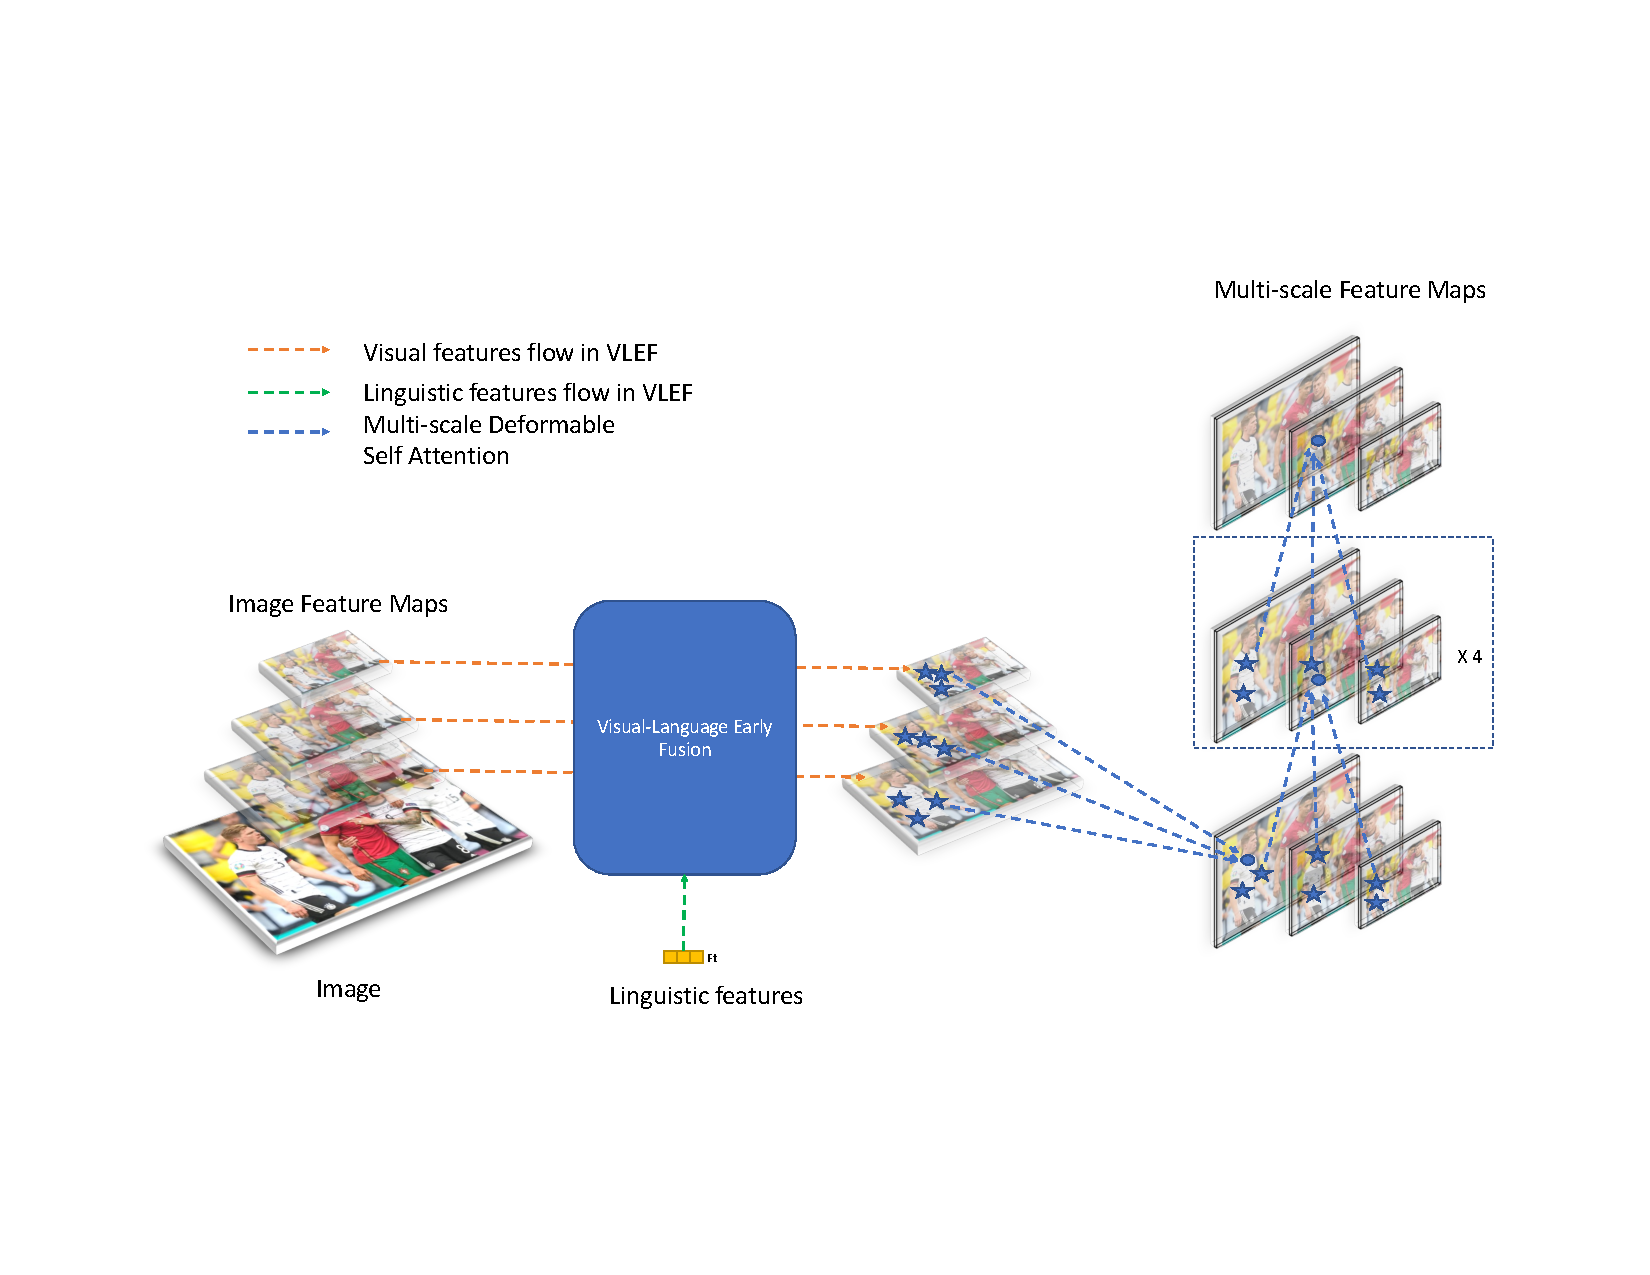
\includegraphics[width=\textwidth]{content/resources/images/referring_segmentation/Cross-modal_Pixel_Decoder.pdf}
    \caption{The overview of Cross-modal Pixel Decoder}
    \label{fig:pixel_decoder}
\end{figure}

\textbf{Pixel Decoder.}
The pixel decoder gradually upsamples the visual features $\hat{F}_v^i$ to generate the fine-grained language-guided visual features $F'_v^i$. 
The Pixel Decoder is adopted from Mask2Former \cite{cheng_masked-attention_2022} with a multi-scale deformable attention module to produce a fine-grained feature pyramid. 

\subsection{Visual-Linguistic Transformer}
\subsubsection{Visual-Linguistic Transformer Block}

\begin{figure}[ht]
    \centering
    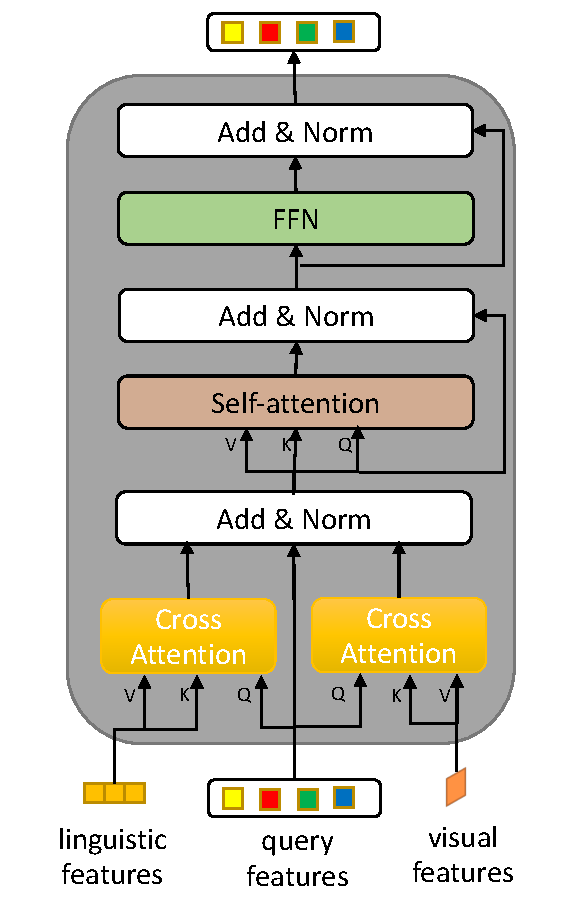
\includegraphics[width=0.5\textwidth]{content/resources/images/referring_segmentation/VLBlock.pdf}
    \caption{The architecture of Visual-Linguistic Transformer Block (VLB). The module takes query features, linguistic features $F_t$ and visual features $F'_v^i$ as input, and generates a better representation of query features.}
    \label{fig:vlb}
\end{figure}

Inspired by the Transformer decoder in Mask2Former \cite{cheng_masked-attention_2022}, we propose a Visual-Linguistic Transformer Block(VLB) to conduct the interaction between queries and visual features and between queries and linguistic features simultaneously. As illustrated in Fig. \ref{fig:vlb}, given the visual features of the video frames, linguistic features of the referring expressions, and the object queries features. 

First, the object queries interact independently with linguistic and visual features in a cross-attention way, where object queries and linguistic/visual features are query and key, respectively. 
And then, they will be summed up and fed into a multi-head self-attention module to update the object queries features and gather the contextual information of both linguistic and visual features. Finally, a FFN module is applied to these features to get the final object query features. 

\subsubsection{Multi-scale features}
Multi-scale features can help the model improve its performance, especially for various object sizes. By utilizing both low-resolution features and high-resolution features in the Transformer decoder layers, the object features can adapt with the size-changing and diversity of object's shapes. 
Specifically, we utilize the features produced by the cross-modal pixel decoder with resolutions 1/32, 1/16, and 1/8 of the original frame. 

In one Transformer decoder layer, there are 3 Visual-Linguistic Transformer blocks. In the first one, the object queries will be updated by the linguistic features and the visual features $F'_3$. In the second VLB block, The updated object queries will be re-updated by the linguistic and the visual features $F'_4$. The last VLB block updates the object queries in the same way but uses the visual feature $F'_5$ instead. 

By repeating these operations multiple times, the final object queries can be adapted with multiple-scale features and can also handle the variety of object sizes in a video. 


\subsection{Instance Matching and Loss}
\label{sec:instance_matching}
Our approach is to generate a small set of $N$ predictions, and the best one will be selected as the final object. In the training phase, therefore, we use the instance matching strategy inspired by ~\cite{cheng_masked-attention_2022, cheng_per-pixel_2021} to supervise candidate instances. 
Let us denote the prediction set as $\hat{y} = \{\hat{y_i}\}_{i = 1}^{N}$, and the prediction for the $i$-th instance is represented by:
\begin{equation}
    \hat{y}_i = \{\hat{p}_i, \hat{s}_i\}.
\end{equation}

For the $i$-th candidate instance, $\hat{p}_i \in \mathbb{R}^1$ is a probability that this instance corresponds to the referred object. Meanwhile, $\hat{s}_i \in \mathbb{R}^{H \times W}$ is the segmentation mask that we predict.

Since there is only one referred object, the ground-truth object is represented as $y \in \mathbb{R}^{H \times W}$. To train the network, we first find the best prediction $i$-th from $N$ candidates via minimizing the matching cost:

\begin{equation}
\begin{split}
    \mathcal{L}_{match}(y, \hat{y}_i) = \gamma_{cls}\mathcal{L}_{cls}(\hat{p}_i, 1) + \gamma_{mask}\mathcal{L}_{mask}(\hat{s}_i, y) \\ + \gamma_{dice}\mathcal{L}_{dice}(\hat{s}_i, y).
\end{split}
\end{equation}
The matching cost is computed based on three loss functions. First, $\mathcal{L}_{cls}$ represents the loss function for the probability a query is the referred object, and we use the Cross-Entropy loss in this work. Second, $\mathcal{L}_{mask}$ is the cross entropy loss that is designed to supervise the mask prediction. Finally, the $\mathcal{L}_{dice}$ is added to improve the dice score, which is quite similar to the IoU metric. 
$\gamma_{cls}, \gamma_{mask}$ and $\gamma_{dice}$ are the coefficients of the three corresponding losses. 

Our goal is to minimize the $\mathcal{L}_{match}$ of one query and maximize the probability of other queries $\hat{p}_j (j \not= i) $ approximate zero (it means these queries do not represent for the referred object). Therefore, our loss function is described as follows: 
\begin{equation}
    \mathcal{L}(y, \hat{y}, i) = \mathcal{L}_{match}(y, \hat{y}_i) + \sum_{\substack{j = 1 \\ j \not=i}}^{N}{\gamma_{cls}\mathcal{L}_{cls}(\hat{p}_j, 0).}
\end{equation}

% \subsection{Instance Sequence Matching and Loss}

% Our approach is to generate the set of $N$ predictions for each frame in $T$ frames. And the $i$-th prediction in all $T$ frames is to track and segment the same object, which is mentioned in \cite{wu_language_2022,cheng_masked-attention_2022}. We can maintain the same relative positions due to sharing object queries between frames. Therefore, we can easily supervise the instance sequence using the instance matching strategy followed \cite{cheng_masked-attention_2022, cheng_per-pixel_2021}. 
% Let us denote the prediction set as $\hat{y} = \{\hat{y_i}_{i = 1}^{N}\}$, and the prediction for the $i$-th instance is represented by:
% \begin{equation}
%     \hat{y}_i = \{\hat{p}_i^t, \hat{s}_i^t\}_{i = 1}^T
% \end{equation}

% For the $t$-th frame, $\hat{p}_i^t \in \mathbb{R}^1$ is a probability that this instance corresponds to the referred object or not. And $\hat{s}_i^t \in \mathbb{R}^{H \times W}$ is the segmentation mask that we predict.

% Since there is only one referred object in the video, the ground-truth instance sequence is represented as $y = \{s^t\}_{t = 1}^T$. To train the network, we first find the best prediction $i$-th from $N$ candidates via minimizing the matching cost:

% % \usepackage{amsmath}
% % \DeclareMathOperator*{\argmax}{arg\,max}
% % \DeclareMathOperator*{\argmin}{arg\,min}

% \begin{equation}
%     \mathcal{L}_{match}(y, \hat{y}_i) = \gamma_{cls}\mathcal{L}_{cls}(\hat{p}_i^t, 1) + \gamma_{mask}\mathcal{L}_{mask}(s_i^t, \hat{s}_i^t) + \gamma_{dice}\mathcal{L}_{dice}(s_i^t, \hat{s}_i^t)
% \end{equation}
% $\mathcal{L}_{cls}$ represents the loss function for the probability a query is the referred object and we use the Cross Entropy loss in this work. $\mathcal{L}_{mask}$ is the binary focal loss that is designed to supervise the mask prediction. And the $\mathcal{L}_{dice}$ is added to improve the dice score, which is quite similar to the IoU metric.
% $\gamma_{cls}, \gamma_{mask}$ and $\gamma_{dice}$ are the coefficients of corresponding losses. 


% Our goal is to minimize the $\mathcal{L}_{macth}$ of one query and the probabilities of other queries $\hat{p}_j (j \not= i) $ approximate zero (it means these queries do not represent for the referred object). Therefore, our loss function is described as follows: 
% \begin{equation}
%     \mathcal{L}(y, \hat{y}, i) = \mathcal{L}_{match}(y, \hat{y}_i) + \sum_{\substack{j = 1 \\ j \not=i}}^{N}{\gamma_{cls}\mathcal{L}_{cls}(\hat{p}_j^t, 0)}
% \end{equation}